%%________________________________________________________________________
%% LERCM | PROJETO
%% 2012 / 2013
%% Modelo para relat�rio
%% v02 (inclui anexo sobre utiliza��o sistema controlo de vers�es)
%% PTS / MAI.2013
%%________________________________________________________________________

\chapter{Diagrama de Atividades}
\label{ch:act}

\section{Diagrama de Atividades - Autentica��o}
\label{sec:act_autenticacao}
%%________________________________________________________________________

\begin{figure}[!ht]
      \centering
      \includegraphics[width=10cm]{Imagens/Atividades/act_autenticacao.pdf}
      \caption{Diagrama de Atividades - Autentica��o}
      \label{fig:act_autenticacao}
\end{figure}

\newpage
\section{Diagrama de Atividades - Registo de Contadores}
\label{sec:act_contadores}
%%________________________________________________________________________

\begin{figure}[!ht]
      \centering
      \includegraphics[width=11cm]{Imagens/Atividades/act_contadores.pdf}
      \caption{Diagrama de Atividades - Registo de Contadores}
      \label{fig:act_contadores}
\end{figure}

%%________________________________________________________________________
\chapter{Modelo Entidade Associa��o da Base Dados}
\label{ch:modeloEAcompleto}
%%________________________________________________________________________

%O \aspas{ap�ndice} utiliza-se para descrever aspectos que tendo sido desenvolvidos pelo autor constituem um complemento ao que j� foi apresentado no corpo principal do documento.
%
%Neste documento utilize o ap�ndice para explicar o processo usado na \textbf{gest�o das vers�es} que foram sendo constru�das ao longo do desenvolvimento do trabalho.
%
%� especialmente importante explicar o objetivo de cada ramo (\aspas{branch}) definido no projeto (ou apenas dos ramos mais importantes) e indicar quais os ramos que participaram numa jun��o (\aspas{merge}).
%
%� tamb�m importante explicar qual a arquitetura usada para interligar os v�rios reposit�rios (\eg, Git, GitHub, DropBox, GoogleDrive) que cont�m as v�rias vers�es (e respetivos ramos) do projeto.
%
%
%Notar a diferen�a essencial entre \aspas{ap�ndice} e \aspas{anexo}. O \aspas{ap�ndice} � um texto (ou documento) que descreve trabalho desenvolvido pelo autor (\eg, do relat�rio, monografia, tese). O \aspas{anexo} � um texto (ou documento) sobre trabalho que n�o foi desenvolvido pelo autor.
%
%Para simplificar vamos apenas considerar a no��o de \aspas{ap�ndice}. No entanto, pode sempre adicionar os anexos que entender como adequados.
%

\begin{figure}[!ht]
      \centering
      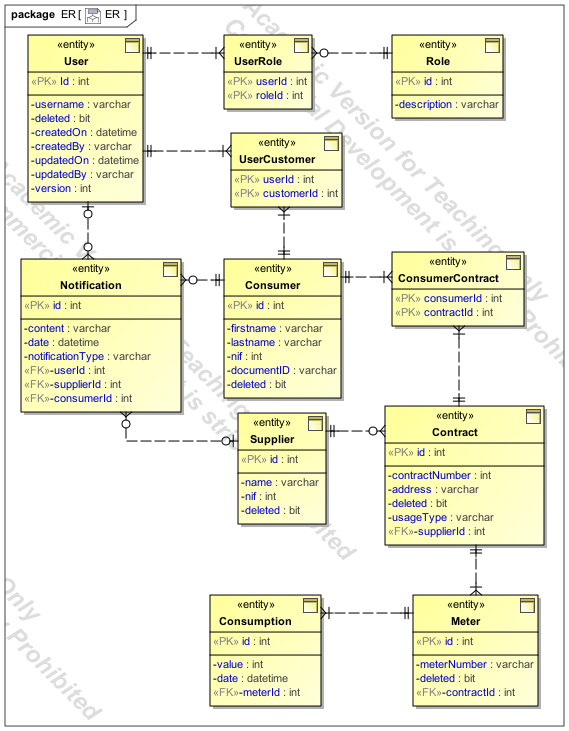
\includegraphics[width=12cm]{Imagens/Modelos/ER.pdf}
      \caption{Modelo Entidade Associa��o da Base de Dados}
      \label{fig:modelo_EA_completo}
\end{figure}




%%________________________________________________________________________
%\chapter{Outro Detalhe Adicional}
%\label{ch:outroDetalheAdicional}
%%________________________________________________________________________

%Escrever aqui o detalhe adicional que melhor explique outro aspecto (diferente do que est� no ap�ndice \ref{ch:umDetalheAdicional}) descrito no corpo principal do documento \ldots









